\section{Разработка конструкции 
  проектируемого изделия} % 4

\subsection{Выбор и обоснование элементной базы,
  конструктивных элементов, 
  установочных изделий, 
  материалов корпуса и защитных покрытий,
  маркировки деталей и сборочных единиц. }

По конструктивному оформлению все ЭРИ (ИЭТ, ЭРЭ и ПМК)
различают~\cite{Belyanin2008}:
\begin{enumerate}
\item корпусные с планарными выводами, лежащими в плоскости основания
корпуса, с осевыми (отформованными) и штыревыми, перпендикулярными
основанию (традиционная элементная база);
\item  корпусные без выводов, с укороченными планарными или j-образными
выводами, уходящими под корпус; в виде матрицы шариковых вводов из
припоя и пр.; их называют микрокорпуса или поверхностно-монтируемые
компоненты (ПМК);
\item  бескорпусные ЭРЭ и ИС.
\end{enumerate}

По конструктивно-технологическому признаку в настоящее время
различают следующие корпуса~\cite{Belyanin2008}:
\begin{enumerate}
\item  металлостеклянные - стеклянное или металлическое основание,
соединенное с металлической крышкой с помощью сварки; выводы
изолированы стеклом;
\item  керамические - керамическое основание и крышка, соединенные
между собой пайкой;
\item  пластмассовые - пластмассовое основание и крышка, соединены
опрессовкой;
\item  металлополимерные - подложка с компонентами и выводами
помещаются в металлическую крышку и герметизируются заливкой
компаундом. Металлическая крышка обеспечивает эффективную влагозащиту,
отвод тепла от кристалла, снижает уровень помех.
\end{enumerate}

Выбор элементной базы производится на основе схемы электрической
принципиальной с учетом изложенных в ТЗ условий и требований.
Эксплуатационная надежность элементной базы в основном определяется
правильным выбором типа элементов при проектировании для использования
в режимах, которые не превышают предельно допустимые~\cite{Alexeev2011}.

Критерием отбора электрорадиоэлементов (ЭРЭ) является соответствие
технических и эксплуатационных характеристик ЭРЭ заданным условиям
работы и эксплуатации ~\cite{Alexeev2011}.

Основными параметрами при выборе ЭРЭ являются ~\cite{Alexeev2011}:
\begin{enumerate}
\item Технические параметры:
  
  \begin{itemize}
  \item номинальное значение параметров ЭРЭ согласно схеме
    электрической принципиальной прибора;
  \item допустимые отклонения величины параметра ЭРЭ от номинального
    значения;
    
  \item допустимое рабочее напряжение ЭРЭ;
    
  \item допустимая мощность рассеивания ЭРЭ; 
  \item диапазон рабочих частот ЭРЭ;
  \item коэффициент электрической нагрузки ЭРЭ;
  \end{itemize}

\item Эксплуатационные параметры:
  \begin{itemize}
  \item диапазон рабочих температур;
  \item относительная влажность воздуха;
  \item атмосферное давление;
  \item вибрационные нагрузки;    
  \item другие показатели.
  \end{itemize}  
\end{enumerate}

Кроме всех выше обозначенных критериев выбора ЭРЭ, активно
применялись принципы стандартизации и унификации ЭРЭ, с
целью получить такие преимущества как улучшение эксплуатационной и
производственной технологичности, снижение себестоимости выпуска
проектируемого изделия и уменьшение сроков проектирования изделия.

% Приведены виды электрорадиоизделий, согласно ~\cite{Belyanin2008}.
% Приведены основные параметры электрорадиоэлементов, согласно
% ~\cite{Alexeev2011}.
% Рассказано на основании каких соображения осуществлялся выбор тех или
% иных элементов.

\subsection{Выбор типа электрического монтажа,
  элементов крепления и фиксации. }

% В этом подразделе рассказано то почему выбран именно THT монтаж в
% данном изделии.
% Тут обосновать использование THT компонентов и зажима устройства в корпус.

Во время проектирования был сделан выбор в пользу того, чтобы размещать
THT компоненты только с одной стороны печатной платы.
Такое решение позволяет ~\cite{yadro-habr-764056}:
% https://habr.com/ru/companies/yadro/articles/764056/
\begin{itemize}
\item в полтора-два раза сократить время монтажа и расходы на трафареты;
\item реже перезаряжать питатели и корректировать термопрофиль;  
\item снизить нагрузку на выходной контроль.
\end{itemize}

Таким образом была повышена простота производства и ремонтопригодности.

Существуют следующие опции при выборе типа монтажа на печатной плате:
\begin{itemize}
\item поверхностный монтаж;
\item выводной монтаж;
\item смешанный монтаж.
\end{itemize}

Появление компонентов с большим числом выводов привело к появлению
планарных компонентов и использованию поверхностного монтажа для их
установки.

В данном проекте отсутствуют компоненты со столь большим числом
выводов. У самого большого по числу выводов компонентов
микроконтроллера ATmega328p всего лишь 28 выводов, а на рынке
представлены DIP корпуса для установки микроконтроллера
монтажом в отверстия.

Широкое распространение поверхностный монтаж получил к концу
восьмидесятых годов. Новизна заключается в использовании вместо
компонентов на выводах, вставляемых в отверстия платы, применение
компонентов припаиваемых к контактным площадкам, сформированным
проводящим рисунком. Планарные компоненты не имеют выводов совсем или
редко имеют короткие выводы. Отсутствие отверстий для установки
компонентов снижает затраты на изготовление платы. Планарные
компоненты унифицированы, в несколько раз меньше, вдвое дешевле
выводных аналогов. Модули, собранные по технологии поверхностного
монтажа имеют плотное размещение компонентов, малое расстояние между
компонентами и контактными площадками. Уменьшение длины проводников
улучшает передачу высокочастотных и слабых сигналов, уменьшается
нежелательная индуктивность и емкость. Планарные радиоэлементы имеют
низкую цену. Поверхностный монтаж сегодня распространен намного шире
монтажа в отверстия. Постоянно снижается себестоимость сборки
~\cite{платы.рф-монтаж}.

Поверхностный монтаж обладает рядом недостатков. Жесткое крепление
компонента за корпус к проводящему рисунку приводит к разрушению
компонентов, подвергающихся воздействию перепадам температур. Модули,
собранные из планарных компонентов боятся перегрева при пайке, сгибов
и ударов. Эти воздействия приводят к трещинам компонентов. Разработчик
печатных плат должен проектировать проводящий рисунок, обеспечивающий
равную скорость нагревания контактов компонента благодаря
симметричности тепловых полей. Технология групповой пайки включает в
себя режим работы оборудования и технологическую оснастку
обеспечивающие одинаковую скорость нагревания контактов каждого
компонента для исключения брака. Требуется точно соблюдать требования
переноса пасты на плату и режим работы паяльного
оборудования. Повышаются требования к транспортировке и хранению
планарных компонентов и материалов для монтажа. Отработка трассировки
проводящего рисунка требует больше средств. Возрастают затраты на
технологическую оснастку при выпуске опытных партий. Ремонт модулей
собранных поверхностным монтажом требует специализированного
инструмента ~\cite{платы.рф-монтаж}.

Данный тип монтажа не был выбран из соображений ремонтопригодности
получаемого изделия.

Ручной выводной монтаж модулей целесообразно использовать в следующих
случаях: применение автоматического оборудования невыгодно из-за
малого объема заказа или сборки нескольких макетных образцов модулей,
платы не подходят для автоматизированного монтажа, при окончательном
монтаже выводных элементов после автоматического монтажа. Сегодня
электроника находится на уровне развития не позволяющем полностью
отказаться от ручных операций монтажа. Монтажник тщательно проверяет
внешний вид каждого компонента перед установкой. При необходимости
выполняется очистка выводов от окислов и лужение выводов. Есть
возможность придания выводам каждого компонента, формы наиболее
оптимальной для установки на плате, обусловленной конструкцией
электронного модуля. Ручная формовка позволяет придать форму выводам
компонентов, облегчающую чтение маркировки~\cite{платы.рф-монтаж}.

Выбор данного типа монтажа в данной плате обусловлен
стремлением повысить простоту производства платы в условиях эксплуатации.


\subsection{Выбор способов обеспечения
  нормального теплового режима устройства
  (выбор способа охлаждения
  на ранней стадии проектирования;
  выбор наименее теплостойких элементов,
  для которых необходимо проведение расчёта). }

% Говорится, что выбрано пассивное охлаждение из-за своей простоты.

% Рассказано почему в качестве наименее теплостойкого элемента будет
% выбран единственный транзистор на плате, либо микроконтроллер. На
% данный момент склоняюсь к выбору транзистора.
Защита от тепловых воздействий это одна из важных задач решаемых в
обеспечении надёжности РЭС.
Насыщение современных технических устройств РЭА различного назначения
заставляет конструкторов уменьшать ее габариты и увеличивать удельные
мощности рассеивания, т.е. мощности, приходящиеся на единицу
поверхности или объема РЭА. Одним из основных направлений в
конструировании РЭА стала комплексная микроминиатюризация, что
приводит к ещё большему увеличению удельной мощности рассеивания
~\cite{Rotkop1976}.

Различают внутренние и внешние тепловые воздействия на РЭА.
Внутренние тепловые воздействия на РЭА в основном зависят от мощности
рассеиваемой её элементами ~\cite{Rotkop1976}.

Защита РЭА от тепловых воздействий осуществляется при помощи ряда
мероприятий. Одним из основных является использование систем
обеспечения теплового режима РЭА (СОТР). СОТР обычно предназначена для
поддержания заданного в технических условиях (ТУ) диапазона температур
на элементах РЭА, чтобы обеспечить ее надежность при определенных
тепловых воздействиях и других специальных требованиях ~\cite{Rotkop1976}.

В радиоэлектронных комплексах СОТР, как правило, являются сложными
системами, состоящими из многих элементов, коммуникаций и несущих
конструктор. В некоторых случаях регулирование температуры в РЭА может
быть достигнуто за счет простейших конструктивных решений,
осуществляющих теплопередачу между элементами РЭА, элементами несущей
конструкции и окружающей средой. Тогда нет смысла рассматривать СОТР
как отдельное изделие и мы будем пользоваться терминами «методы (или
способы) охлаждения РЭА». Этими же терминами будем пользоваться и при
исследовании температурного поля элементов РЭА, в результате действия
некоторых гипотетических СОТР, когда конкретная конструкция СОТР не
рассматривается ~\cite{Rotkop1976}.

Для выбора и обоснование системы охлаждения важно иметь представление
о тепловом режиме РЭС.  Тепловой режим есть совокупность значений
температур в различных точках всей РЭС, её корпуса и СОТР.

Тепловой режим РЭА характеризуется, прежде всего, двумя факторами:
электрическим режимом работы и условиями эксплуатации ~\cite{Rotkop1976}.

Энергетический коэффициент полезного действия радиоэлементов, как
правило, невелик, и значительная доля энергии питания превращается в
тепловую энергию с сопутствующим перегревом элементов и аппаратуры
~\cite{Rotkop1976}.


Электрический режим работы РЭА в данном случае интересует нас только в
связи с изменением внутренних тепловых воздействий во времени и
пространстве и задается обычно в виде графиков зависимости
рассеиваемой мощности от времени для различных узлов РЭА~\cite{Rotkop1976}.

Из технического задания известно, что режим работы данного РЭС —
длительный. То есть устройство работает в течении достаточно большого
периода времени рассеивая постоянную по величине мощность.

Такой электрический режим не позволит использовать радиаторы в виде
так называемых тепловых аккумуляторов.

Данные касаемо условий эксплуатации были приведены ранее и
соответствуют условиям категории УХЛ 4.2 указанным в ГОСТ
~\cite{GOST-15150-69}.

Понятию «достаточно большой промежуток времени» в контексте охлаждения
РЭС соответствует такой промежуток времени, за который полностью
устанавливается тепловой режим этого РЭС.

Учитывая тип и состояние теплоносителя, также причину, вызвавшую его
движение, способы охлаждения РЭА можно разделить на следующие основные
классы: газовое (воздушное), жидкостное, испарительное, а также
естественное и принудительное ~\cite{Rotkop1976}.

Здесь некоторый способ охлаждения может относиться сразу к двум
классам: по агрегатному состоянию теплоносителя и тому принудительно
ли осуществляется охлаждение.

Естественное воздушное охлаждение РЭА является наиболее простым,
надежным и дешевым способом охлаждения и осуществляется без затраты
дополнительной энергии. Однако интенсивность такого охлаждения
невелика, поэтому использование этого способа возможно при небольших
удельных мощностях рассеивания (мощностях, рассеиваемых
единицей поверхности или объема), т.е. в РЭА, работающей в облегченном
тепловом режиме. При естественном воздушном охлаждении конвективный
теплообмен осуществляется за счет энергии,
рассеиваемой элементами РЭА ~\cite{Rotkop1976}.

Естественное воздушное охлаждение РЭА с перфорированным кожухом
позволяет обеспечить тепловой режим при более высоких удельных
мощностях рассеивания, чем при герметичном кожухе ~\cite{Rotkop1976}.

Однако в таком случае, ухудшаются показатели защищенности устройства
от пыли.

Расчет теплового режима радиоэлектронных аппаратов рекомендуется
проводить в три этапа~\cite{Rotkop1976}:
\begin{enumerate}[label={\arabic*.}]
  \item Определение среднеповерхностной температуры платы с
расположенными ней деталями, корпуса и температуры воздуха внутри
радиоэлектронного аппарата.
  \item Определить среднеповерхностные температуры корпусов элементов
  используя результаты первого этапа.
  \item Определить максимальные температуры критических зон элементов и
их функциональные связи со среднеповерхностной температурой как
корпусов, так и и плат.
\end{enumerate}

Первый и второй этапы расчета позволяют получить значения основных
параметров, связанных с выбором системы охлаждения, т.е. первых двух
этапов хватает для принятия конструкторского решения касаемо выбора
системы охлаждения.

Полную систему уравнений теплообмена для реального аппарата часто
невозможно не только решить аналитически, но и строго записать. В
связи с этим процессы, протекающие в реальном радиоэлектронном
аппарате, схематизируют, принимают ряд упрощающих предпосылок и в
результате получают тепловую модель аппарата, для которой и проводят
расчет теплового режима ~\cite{Rotkop1976}.

Наибольшее распространение получила весьма плодотворная схематизация
процессов теплообмена в РЭА, предложенная Г.Н.Дульневым
~\cite{Dulnev1968}.

Суть метода заключается в том, что печатная плата с её элементами
принимается за одно тело с изотермической поверхностью (нагретую
зону), для которого и проводится расчет теплового режима.

Таким образом производится расчет среднеповерхностной температуры
нагретой зоны.

Под понятием нагретая зона понимается поверхность того элемента на
печатной плате, который рассеивает больше всего мощности.

Во всей схеме практически не встречаются компоненты с большим
тепловыделением. Так например найти коэффициент TDP для
микроконтроллера не представляется возможным, потому что среди
производителей микроконтроллеров, в отличие от производителей
микропроцессоров не принято не то что рассчитывать этот коэффициент
рассеивания теплоты, а даже закладывать в этот компонент схемы
возможности какого-либо его нагрева.

Однако это ни в коем случае не означает то, что ни один из элементов
не будет нагреваться. Напротив при работе любого электронного прибора
какая-то часть потребляемой мощности рассеивается как тепло.

Но если рассматривать отношение мощности потребляемой и рассеиваемой
как тепло, то можно понять, что самым простым оно будет у резисторов.

По видимому, можно взять информацию о мощности резистора и принять её
за мощность рассеиваемую в виде теплоты
~\cite{HeatDissipatedResistors}.

Примерно таким же образом было сделано допущение о схожести в вопросе
рассеиваемой мощности между резисторами и потенциометрами.

В принципе задача теплоотвода — удерживать переходы транзисторов или
других устройств при температуре, не превышающей указанной для них
максимальной рабочей температуре. Для кремниевых транзисторов в
металлических корпусах максимальная температура переходов обычно равна
200°C, а для транзисторов в пластмассовых корпусах 150°С
~\cite{ArtOfElectronics2010}.

Зная нужные параметры,
проектировать теплоотвод просто~\cite{ArtOfElectronics2010}:
Зная мощность, которую прибор будет рассеивать в данной схеме,
подсчитываем температуру переходов с учетом теплопроводности
транзистора, радиатора и максимальной рабочей температуры окружающей
транзистор среды. Затем выбираем такой радиатор, чтобы температура
переходов была максимально ниже указанной изготовителем
максимальной. Здесь разумно перестраховаться, так как при температурах
близких к максимальной, транзисторы быстро выходят
из строя~\cite{ArtOfElectronics2010}.

Однако, стоит заметить, что установка дополнительного радиатора
это увеличение количества компонентов, которые могут отказать, то есть,
если возможно, то такого искусственного увеличения количества компонентов
следует избегать.

Из вышеизложенного можно сделать вывод, что в качестве наименее
теплостойких элементов для которых нужно производиться расчёт следует
выбрать транзистор. Если хочется сделать расчёт более простым, то
выбрать стоит резисторы, взяв за основу потенциометры.

% Обоснование почему охлаждать необходимо транзистор, а не микроконтроллер.

\subsection{Выбор и обоснование
  метода изготовления печатной платы. }

% В данном разделе будет приведена информация про несколько оптимальных
% с разных точек зрения методов изготовления печатный платы. Будет
% указано почему выбран один конкретный метода. На данный момент таким
% методом выбран метод фрезерования ~\cite{PirogovaEngineering}.

Оптимальным же с точки зрения изготовления было бы проектирование
двухсторонней ПП с использованием метода фрезерования.

Этот механический метод применяют при единичном изготовлении ДПП
полностью на одном универсальном станке фирм, например, LPKF, Bungard,
VHF, Mitronic~\cite{PirogovaEngineering}.
Он включает следующие этапы:
\begin{enumerate}
\item подготовка управляющего файла для станка;
  
\item сверление монтажных и переходных отверстий по программе;
\item фрезерование (высвобождение) мест от фольги твердосплавными коническими фрезами
  с углом при вершине 60 или 30 град.
  Файл оконтуривания генерируется в одной из программ CAD-CAM
  (InstantCAM, CircuitCAM, САМ 350);
  
\item металлизация монтажных и переходных отверстий.

\end{enumerate}

Применяя фрезу с рабочим диаметром 100 мкм, изготавливают ДПП по 4-му
классу точности, т.е. между выводами ЭРИ со стандартным шагом 2,54 мм
можно провести пять проводников.  При этом основным требованием,
предъявляемым к материалу ДПП, является плоскостность.  Для исключения
разброса ширины реза при фрезеровании применяют специальные прижимные
головки.  При этом контролируют глубину врезания фрезы в заготовку и
равномерность прижима заготовки к рабочему столу.

Металлизацию переходных отверстий осуществляют пустотелыми заклепками;
обслуженными пустотелыми заклепками, содержащими припой с флюсом,
которые вставляют в отверстие, и с помощью паяльника расплавляют
припой; специальными пастами, которые разогревают в
печах при температуре $160 \pm 10$°C.

Основными преимуществами механического способа являются высокая
оперативность и простота реализации, а недостатками — низкая
производительность и высокая стоимость
оборудования~\cite{PirogovaEngineering}.

\subsection{Выбор конструкторских решений, 
  обеспечивающих удобство ремонта
  и эксплуатации устройства.}

По ГОСТ 23751-86 предусмотрены следующие типы конструкции ПП
~\cite{PirogovaEngineering}:
\begin{enumerate}

\item Односторонние ПП. Применяются в бытовой технике, технике связи и
  в блоках питания на ЭРЭ. Имеют низкую стоимость, высокую надежность,
  низкую плотность компоновки;

\item двусторонние ПП. Применяются в измерительной, вычислительной
  технике, технике управления и автоматического регулирования,
  технике связи, высокочастотной технике;

\item многослойные ПП. Применяются в технике управления и
  автоматического регулирования,
  вычислительной и бортовой аппаратуры для
  коммутации ИМС, БИС, СБИС, МСБ, в ЭА с высокими требованиями по быстродействию,
  плотности монтажа,  волновому сопротивлению, времени задержки сигнала и т.д.;

\item гибкие ПП, ГЖП и ГПК. Применяются в ЭА и высокой надежности
  при реализации уникальных и сложных технических решений,
  конструкция которых исключает применение жестких ПП.
\end{enumerate}

Чем больше слоев, тем легче трассировать печатную плату.
Однако большее число слоёв затрудняет производство печатной платы
в условиях лаборатории, в которых может использоваться разрабатываемое
устройств.

Оптимальным с точки зрения трассировки было бы проектирование
многослойной печатной платы, с четырьмя слоями, при этом на первом
внутреннем слое полигон земли, а на втором полигоны питания.

В итоге был выбран вариант проектирования с двухсторонней печатной платой,
ввиду доступности изготовления ПП таким способом в условиях её
эксплуатации.

% Рассказано о том, как  может быть осуществлено перепрограммирование устройства с
% помощью разъёма ISP, без выпаивания микроконтроллера из печатной
% платы. Обосновывается выбор THT компонентов, как облегающих ремонт.
% Возможно, обосновывается добавление резистора, находящегося
% между транзистором и микроконтроллером, как меры безопасности.

\subsection{Технология разработки чертежа детали в среде KiCAD.}
Из-за приверженности к свободному программному обеспечению
~\cite{GNU-philosophy}, для создания проекта печатной платы была
выбрана САПР с открытым исходным кодом KiCAD
~\cite{kicad-license}.

Такой выбор связан, этическими соображениями, которые, будучи
кратко сформулированы, звучат как:
Если пользователи не контролируют программу,
программа контролирует пользователей ~\cite{unfair-nonfree-programms}.

Для того, чтобы пользователи контролировали программу, требуется
четыре фундаментальные свободы~\cite{unfair-nonfree-programms}:

\begin{enumerate}
\item Свобода выполнять программу как вам угодно, в любых целях;
  
\item Свобода изучать «исходный текст» программы и править его, чтобы
программа проводила ваши вычисления как вам угодно. Программы пишутся
программистами на языках программирования (сочетающих естественные
языки с алгеброй) — и это образует форму программы, которую называют
«исходный текст». Всякий, кто умеет программировать и у кого есть
программа в форме исходного текста, может прочесть исходный текст и
понять, как она работает, а также внести изменение. Когда все, что у
вас есть — это исполняемая форма, последовательность чисел, которые
компьютер эффективно выполняет, но которые человеку понимать крайне
трудно, то разбираться в программе и править ее в этом виде трудно до
невозможности.

\item  Свобода копировать и распространять свободные копии когда вам
угодно. (Это не обязанность; вы делаете это по своему выбору. Если
программа свободна, это не значит, что кто-то обязан предлагать вам
копию или что вы обязаны предлагать копию ему. Распространение
программы среди пользователей без свободы несправедливо по отношению к
ним; однако решение не распространять программу — пользоваться ею
частным порядком — не сопряжено с несправедливостью в отношении
кого-либо.)

\item Свобода копировать и распространять свои измененные версии когда
вам угодно.
\end{enumerate}

Другая причина выбора данной САПР при разработке, используемый в ней,
текстовой формат файлов, при котором данные в документах САПР
представлены не иначе как Эс-Выражения (англ. S-Expressions)
~\cite{kicad-sexpr}.

% \begin{figure}[H]
%   \centering
%   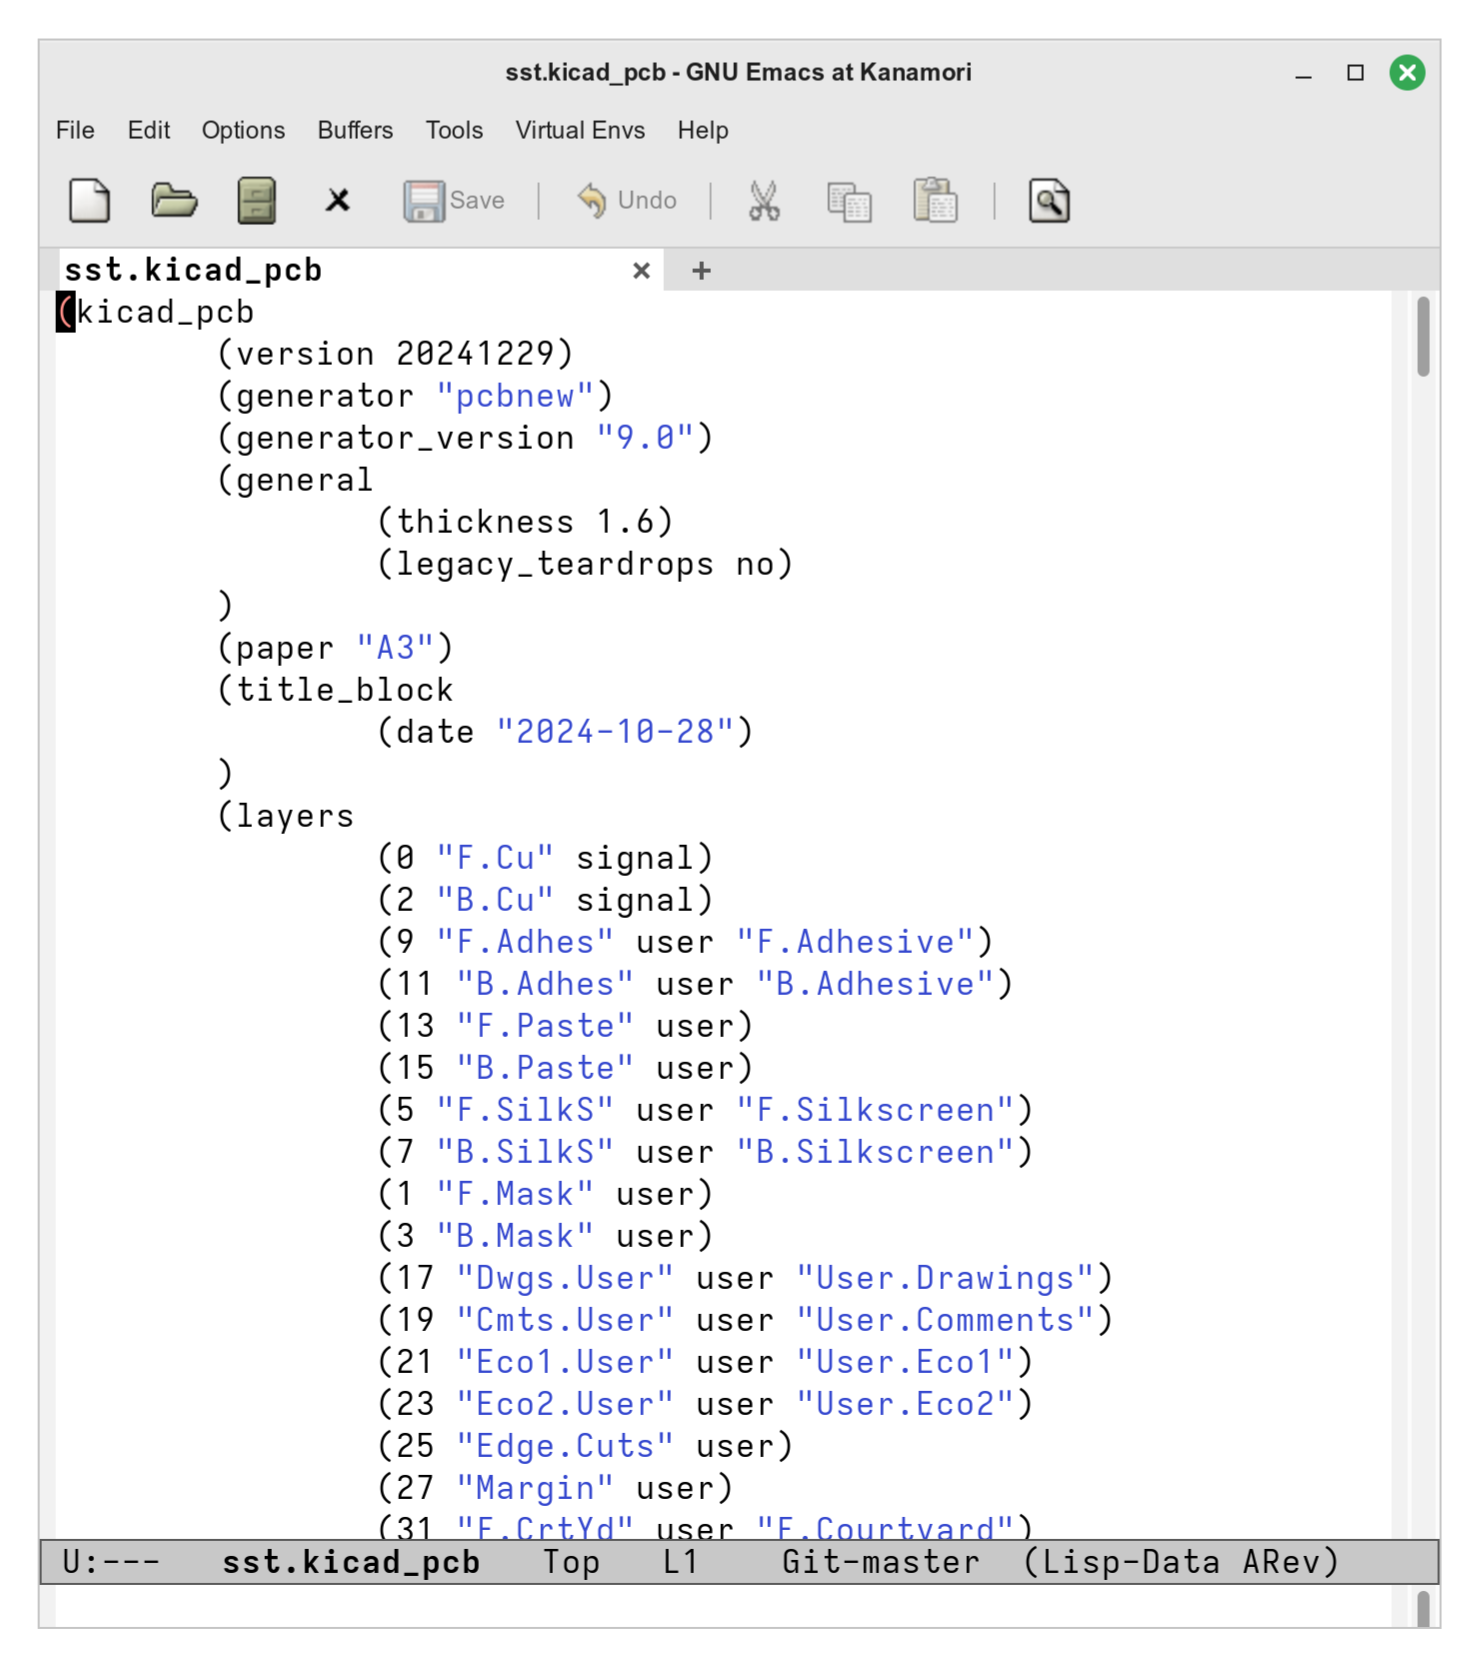
\includegraphics[scale=0.15]{kicad/emacs-pcbdoc.png}
%   \caption{Скриншот файла печатной платы KiCAD открытого в текстовом редакторе}
% \end{figure}


В отличие от бинарных файлов, используемых в Altium Designer, файлы
созданные при разработке печатной платы, в KiCAD за счёт использования
в них текста возможно разместить в репозитории системы контроля версий
git.

Git это распределённая система контроля версий 
исходного кода \cite{git-dvcs}.

Из-за формата, файлы KiCAD могут быть обработаны, как исходный код.
Это даёт возможность удобной кооперации, при совместной работе.

Например в едином репозитории печатной платы, один конструктор в
соответствующем файле создаёт принципиальную схему устройства, а
другой, в свою очередь, синхронизировав изменения репозитория через
git, используя готовую схему, трассирует печатную плату.

Более того, используя, так называемый монорепозиторий, как подход
работы с git, в одном репозитории можно содержать как печатную плату,
так и исходный код прошивки микроконтроллера, используемый в ней.

Для разработки печатной платы данного электронного модуля было
достаточно использование САПР ПП KiCAD, однако стоит отметить, что
использование специальных САПР симуляторов, например Proteus или
SimulIDE позволяет промоделировать работу принципиальной схемы,
используемой в ПП, а также получить информацию нужную, для
вычисления коэффициента нагрузки устройства $K_{Н}$ при расчете
надёжности.


Большую сложность при выполнении работы составила необходимость
выполнять чертёж платы.

Интерфейс KiCAD-pcbdoc рассчитан под трассировку печатной платы, но
никак не под черчение отдельного чертежа.  Присутствует возможность
редактировать форматную рамку, наносить разнообразные размеры, чертить
на пользовательском слое.  Однако возможности выделить каждый слой
платы как отдельный вид на чертеже нет.

Тем не менее в KiCAD присуствует возможность послойного экспорта в dxf
слоёв разрабатываемой печатной платы.

\begin{figure}[H]
  \centering
  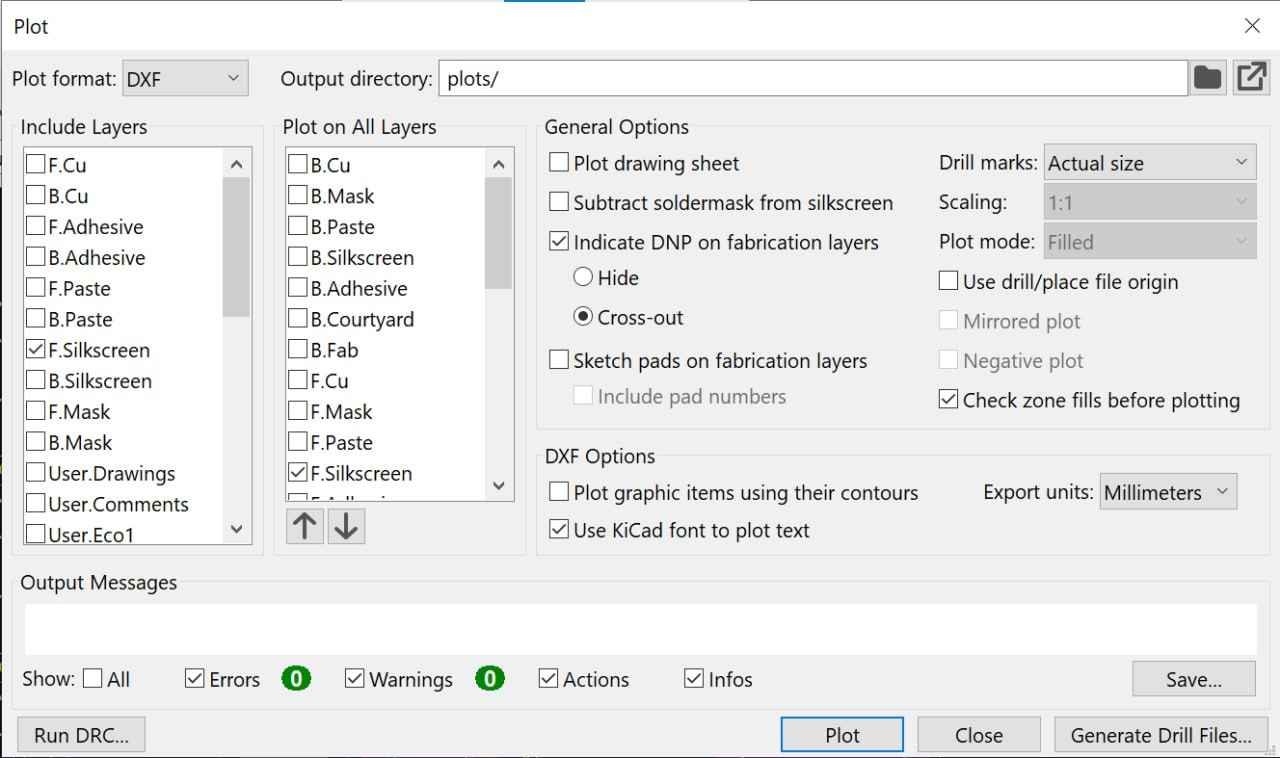
\includegraphics[scale=0.5]{kicad/dxf-export.jpg}
  \caption{Скриншот окна экспорта dxf САПР KiCAD}
\end{figure}

Эта возможность и была использована для создания чертежа платы в
программе Autodesk AutoCAD. Нужные слои печатной платы были
экспортированы в dxf из KiCAD, а затем импортированы в AutoCAD. В
дальнейшем, выполнение чертежа ПП осущствлялось в Autodesk AutoCAD c
применением нативного формата DWG.

CALS (continuous acquisition and lifecycle support)  — это
непрерывная информационная поддержка жизненного цикла продукта.
Внедрение CALS-технологий на предприятии обычно
предполагает~\cite{Lanin2019}:
\begin{enumerate}
\item Полное реформирование процессов на предприятии, включая
проектирование, конструирование, подготовку, производства, закупки,
производство, управление, материально-техническое снабжение, сервисное
обслуживание;

\item Использование современных информационных технологий;
  
\item Совместное использование данных, полученных на различных стадиях
  жизненного цикла продукта;
  
\item Применение международных стандартов в области информационных
технологий в целях интеграции, совместного использования информации и
управления ею.
\end{enumerate}

Была внедрены следующая CALS-технологии – Файлы STEP для экспорта
трехмерной модели печатной платы, которая использовалась при
моделировании и для того, чтобы разработать корпус платы.


% Рассказано, как разработан чертёж принципиальной схемы и печатные
% платы в САПР KiCAD. Обоснован выбор именно свободного ПО, типа САПР
% KiCAD.  Рассказано как проходит разработка в данной САПР, а также как
% может осуществляться контроль разрабатываемых файлов с помощью git.

\subsection{Обеспечение требований стандартизации, 
  унификации и технологичности конструкции устройства.}

% Приведены ГОСТы из листа задания. Рассказано о том, что именно
% предпринималось, чтобы изделия соответствовало данным нормативным
% документам.

Создание современных технических устройств предполагает не только
разработку эффективной и работоспособной конструкции, но и
обязательное соблюдение целого ряда принципов, направленных на
упрощение и оптимизацию процессов проектирования, изготовления, сборки
и эксплуатации изделий. К числу таких принципов относятся
стандартизация, унификация и технологичность конструкции.

Внедрение данных принципов на этапе конструкторской проработки
позволяет снизить трудоемкость производства, уменьшить издержки,
обеспечить взаимозаменяемость элементов и улучшить эксплуатационные
характеристики устройства. Кроме того, это способствует сокращению
сроков проектирования и снижению вероятности ошибок при разработке и
производстве изделий.

Стандартизация представляет собой процесс установления и применения
единых норм, требований и правил в области проектирования,
производства и эксплуатации изделий. В контексте конструкторской
деятельности она предполагает:

\begin{itemize}
\item использование стандартных элементов, компонентов и материалов,
\item cоблюдение требований государственных,
  отраслевых и международных стандартов,
\item  оформление конструкторской документации по единой системе.
\end{itemize}

Данный показатель предполагает обеспечение качества продукции в
соответствии с уровнем развития науки, техники и технологии;
Стандартизация направлена на достижение оптимальной степени
упорядочения в определенной области посредством установления положений
для всеобщего и многократного применения в отношении реально
существующих или потенциальных задач.

Современная стандартизация базируется на следующих принципах:
\begin{itemize}
\item системность,  
\item повторяемость, 
\item вариантность,
\item  взаимозаменяемость.
\end{itemize}

Системность предполагает обеспечение взаимной согласованности,
непротиворечивости, унификации и исключение дублирования требований
стандартов.

Повторяемость определяет круг объектов, к которым применимы вещи,
процессы, отношения, обладающие общим свойством.

Вариантность предполагает обеспечение минимума рациональных
разновидностей стандартных элементов, входящих в стандартизируемый
объект.

Взаимозаменяемость предусматривает возможность сборки или замены
одинаковых деталей, изготовленных в разное время и в различных местах.

Унификация - это приведение различных видов продукции и средств её
производства к рациональному минимуму типоразмеров, марок, форм и
свойств. Основной целью унификации является устранение неоправданного
многообразия изделий одинакового назначения и разнотипности их
составных частей и деталей, приведение к возможному единообразию
способов их изготовления, сборки и испытаний~\cite{Lanin2019}

Грамотно спроектированное изделие должно одновременно соответствовать
всем трем принципам.

Унификация может осуществляться на различных уровнях:
\begin{itemize}
\item повысить качество выпускаемой продукции;
\item упростить процессы сопровождения и ремонта;
\item добиться экономической эффективности на всех стадиях жизненного цикла.
\end{itemize}

При анализе проектируемого устройства по перечисленным выше
показателям были сделаны выводы о том, что изделие соответствует
необходимым требованиям. Так, например, электрическая схема априорно
технологична ввиду содержания максимального количества унифицированных
узлов (что видно на принципиальной и структурной электрических схемах)
и серийно выпускаемых электроэлементов. Также в электрической схеме
устройства отсутствуют элементы не серийного производства. За счет
использования максимально возможного количества элементов
поверхностного монтажа количество отверстий сведено к минимуму, что
сводит к минимуму затраты ресурсов и энергии при производстве. Все
вышеперечисленное доказывает и соответствие требованиям
стандартизации. Схему можно разбить на отдельные функциональные узлы,
каждый из которых выполняется на плате печатного монтажа,
унифицированного размера в соответствие с существующими стандартами,
при этом основание платы изготавливается по типовому технологическому
процессу, освоенному в производстве.

Корпус изделия также изготавливается в соответствии с требованиями
стандартизации и унификации, однако степень его технологичности ниже
из-за необходимости соединения деталей корпуса при помощи крепежных
элементов.

Таким образом, можно сделать вывод о том, что система автоматического
управления беспилотным летательным аппаратом мультироторного типа
обладает высоким показателем технологичности и соответствует
требованиям стандартизации и унификации.

\newpage


%%% Local Variables:
%%% mode: LaTeX
%%% TeX-master: "main"
%%% LaTeX-biblatex-use-Biber: t
%%% End:
